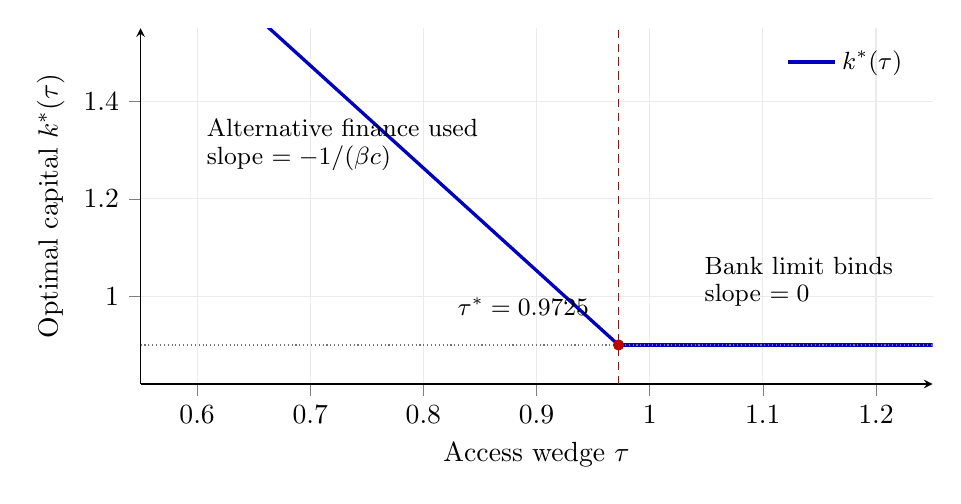
\begin{tikzpicture}
\begin{axis}[
  width=0.96\linewidth,
  height=6.1cm,
  xmin=0.55, xmax=1.25,
  ymin=0.82, ymax=1.55,
  xlabel={Access wedge $\tau$},
  ylabel={Optimal capital $k^*(\tau)$},
  axis lines=left,
  tick align=outside,
  grid=major,
  grid style={draw=black!8},
  legend style={draw=none, fill=none, font=\small,
    at={(0.98,0.97)}, anchor=north east},
  clip=true,
]
  \addplot[blue!75!black, very thick, domain=0.55:0.9725, samples=80]
    {(1.4-x)/0.475};
  \addplot[blue!75!black, very thick, domain=0.9725:1.25, samples=2]
    {0.9};
  \addlegendentry{$k^*(\tau)$}

  \addplot[red!75!black, densely dashed]
    coordinates {(0.9725,0.82) (0.9725,1.55)};
  \addplot[black!55, densely dotted]
    coordinates {(0.55,0.9) (1.25,0.9)};
  \addplot[only marks, mark=*, mark size=1.8pt, red!75!black]
    coordinates {(0.9725,0.9)};

  \node[anchor=south east, font=\small] at (axis cs:0.955,0.94)
    {$\tau^*=0.9725$};
  \node[anchor=west, align=left, font=\small] at (axis cs:0.60,1.31)
    {Alternative finance used\\[-1pt]slope $=-1/(\beta c)$};
  \node[anchor=west, align=left, font=\small] at (axis cs:1.04,1.03)
    {Bank limit binds\\[-1pt]slope $=0$};
\end{axis}
\end{tikzpicture}
